\documentclass[paper=a4, fontsize=11pt]{article}

%code syntax highliter
\usepackage[usenames,dvipsnames]{color,xcolor}
\usepackage{listings}

\usepackage{setspace}
\usepackage{wrapfig}
\usepackage{caption}
\usepackage{mathtools}
\usepackage[hidelinks]{hyperref}
\usepackage{fancyhdr}
\usepackage{array} % "m'' used in tabular env.

\usepackage{tikz}
\usetikzlibrary{shapes.geometric}
\usetikzlibrary{calc}
\usetikzlibrary{positioning}
\usepackage{tikz-qtree}

\usepackage{pgfplots}
\pgfplotsset{compat=1.13} % Nicer axis label placement

\usepackage{cleveref}
\usepackage{graphicx}
\graphicspath{ {../../../formats/globals/} {images/}}

\usepackage{tikz,lmodern}
\usepackage[most]{tcolorbox}

\usepackage{xepersian}
\settextfont{Vazir}
\setlatintextfont{Vazir}

\newcommand{\diam}[1]{\tikz\draw (0,0)node[shape aspect=1,diamond,draw,,inner sep=2pt]{#1};} % Diamond



%%%% START‌ Box %%%%
\newenvironment{questionbox}{
\begin{tcolorbox}[colback=red!5!white,colframe=red!75!black]
}{
\end{tcolorbox}
}
%%%% END‌ Box %%%%

%%%%% Start Pages Config %%%%%%
\pagestyle{fancy}
\rhead{ پاسخ تمارین | مبانی هوش }
\lhead{ علی فرجی}
\cfoot{ \diam{\thepage} }
%%%%% End Pages Config %%%%%%

%%%%%% syntax highliter settings %%%%
\lstdefinestyle{customc}{
  belowcaptionskip=1\baselineskip,
  breaklines=true,
  frame=L,
  xleftmargin=\parindent,
  language=C,
numbers=left,
showspaces=false,           % Leerzeichen anzeigen ?
showtabs=false,             % Tabs anzeigen ?
  showstringspaces=false,
xleftmargin=25pt,
xrightmargin=10pt,
framexleftmargin=17pt,
framexrightmargin=5pt,
framexbottommargin=4pt,
  basicstyle=\footnotesize\ttfamily\setstretch{.8},
  keywordstyle=\bfseries\color{green!40!black},
  commentstyle=\itshape\color{purple!40!black},
  identifierstyle=\color{blue},
  stringstyle=\color{orange},
}
%%%%%% syntax highliter settings %%%%

\begin{document}
\thispagestyle{empty}
\setstretch{2}
	\begin{titlepage}
		\begin{center}
		
       \vspace*{1cm}
       
       \textbf{مبانی و کاربرد های هوش مصنوعی}

       \vspace{0.5cm}
       
پاسخ تمارین سری دوم
       \vspace{2cm}
       

	\textbf{علی فرجی 9634024}
       
       \vspace{2cm}
       
استاد درس: دکتر سیده فاطمه موسوی
 \vfill

     \includegraphics[width=0.4\textwidth]{aut}
 
دانشگاه صنعتی امیرکبیر (پلی تکنیک تهران) \\
دانشکده مهندسی کامپیوتر\\
\today

   \end{center}
\end{titlepage}

\tableofcontents
\thispagestyle{empty}

\newpage

\setcounter{page}{1}

\section{سوال اول}
\subsection{بخش الف}
فضای حالت را می توان به صورت
$(x,y,d,v)$
نشان داد که d جهت (بالا، پایین، چپ، راست)، v سرعت، x و y هم که مختصات خودرو هستند.

اندازه فضای حالت برابر $ M * N * (V_m + 1) * 4 $ خواهد بود.

\subsection{بخش ب}
در هر مرحله یا سرعت بیشتر از صفر است که نمی تواند کاری جز دو عمل افزایش و کاهش و حتی اگر حداکثر سرعت باشد، کاهش سرعت انجام دهد.

اگر هم سرعتش صفر باشد می تواند دور زدن ها و یا افزایش سرعت را انجام دهد که در این صورت حداکثر تعداد فرزندان 3 می شود.

پس حداکثر ضریب انشعاب 3 است.

\section{سوال دوم}
\subsection{بخش الف}
فرض می کنیم کوتاه ترین مسیر همان کم هزینه ترین مسیر است:

گراف جستوجوی \lr{UCS} به صورت زیر می شود:
\begin{center}
\rotatebox{270}{%
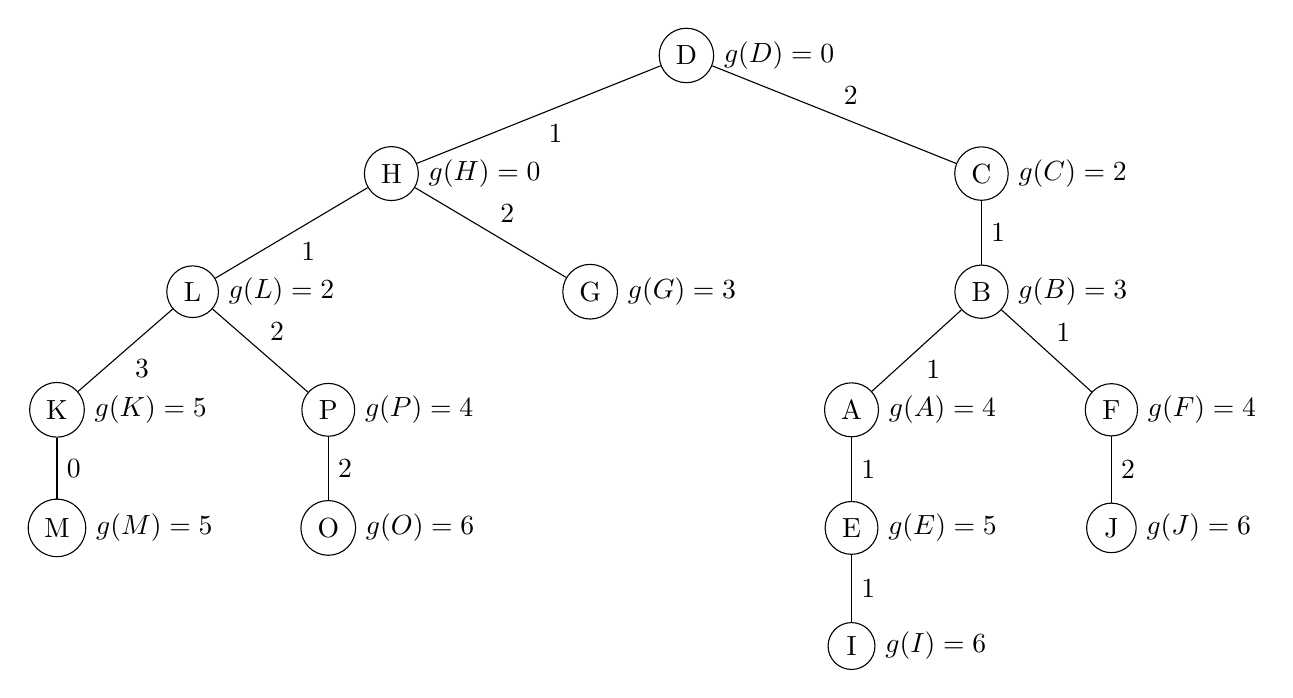
\begin{tikzpicture}[every tree node/.style={draw,circle},
   level distance=1.5cm,sibling distance=1cm,
   edge from parent path={(\tikzparentnode) -- (\tikzchildnode)}]
\Tree
[.\node [label={right:$g(D)=0$}] {D}; 
	\edge node[auto] {1};
	[.\node [label={right:$g(H)=0$}] {H}; 
		\edge node[auto] {1};
		[.\node [label={right:$g(L)=2$}] {L}; 
			\edge node[auto] {3};
			[.\node [label={right:$g(K)=5$}] {K}; 
	       		\edge node[auto] {0};
	       		[.\node [label={right:$g(M)=5$}] {M};  ]
			]
	       	\edge node[auto] {2};
	       	[.\node [label={right:$g(P)=4$}] {P}; 
	       		\edge node[auto] {2};
	       		[.\node [label={right:$g(O)=6$}] {O};  ]
	       	]
		 ]
		\edge node[auto] {2};
		[.\node [label={right:$g(G)=3$}] {G};  ]
	]
	\edge node[auto] {2};
	[.\node [label={right:$g(C)=2$}] {C};  
		\edge node[auto] {1};
		[. \node [label={right:$g(B)=3$}] {B};  
			\edge node[auto] {1};
			[.\node [label={right:$g(A)=4$}] {A}; 
	       		\edge node[auto] {1};
	       		[.\node [label={right:$g(E)=5$}] {E};  
		       		\edge node[auto] {1};
		       		[.\node [label={right:$g(I)=6$}] {I};  ]
	       		]
			]
	       	\edge node[auto] {1};
	       	[.\node [label={right:$g(F)=4$}] {F};  
	       		\edge node[auto] {2};
	       		[.\node [label={right:$g(J)=6$}] {J};   ]
	       	]
		 ]	
	]
]
\end{tikzpicture}}

\end{center}

\newpage
تغییرات مجموعه مرزی و کاوش شده:

\begin{center}
\begin{latin}
\begin{tabular}{ |c|c| } 
\hline
Frontier & Explored \\
\hline
D(0) &   \\ 
H(1), C(2) & D \\ 
G(3), L(2), C(2) & D, H \\ 
G(3), L(2), B(3) & D, H, C \\ 
G(3), P(4), K(5), B(3) & D, H, C, L \\ 
G(3), P(4), K(5), F(4), A(4) & D, H, C, L, B \\ 
P(4), K(5), F(4), A(4) & D, H, C, L, B, G \\ 
P(4), K(5), F(4), E(5) & D, H, C, L, B, G, A \\ 
P(4), K(5), J(6), E(5) & D, H, C, L, B, G, A, F\\ 
O(6), K(5), J(6), E(5) & D, H, C, L, B, G, A, F, P\\ 
O(6), K(5), J(6), I(6) & D, H, C, L, B, G, A, F, P, E\\ 
O(6), M(5), J(6), I(6) & D, H, C, L, B, G, A, F, P, E, K\\ 
\hline
\end{tabular}
\end{latin}
\end{center}

بعد از مرحله آخر میریم که M را گسترش دهیم ولی قبل از گسترش چک می کنیم که این هدف است یا خیر که می بینیم این گره هدف است و تمام.


\subsection{بخش ب}
اگر در خانه حاشیه حرکت کنیم حداکثر 2 مسیر داریم یکی به سمت داخله یکی به سمت جلو (خانه قبلی نمی توانیم برویم)

اگر در وسط حرکت کنیم فقط به خانه قبلی نمی توانیم برویم و حداکثر 3 مسیر پیش رو داریم.

اگر در وسط به سمت یک هتل تفریحی حرکت کنیم علاوه بر حالت بالا یک حالت پرواز با هلیکوپر هم خواهیم داشت.

پس در این نوع مساله حداکثر ضریب انشعاب 4 است.

\section{سوال سوم}
\subsection{بخش الف}
با در نظر گرفتن یال های جهت دار:

گره \lr{Goal2} به عنوان هدف پیدا خواهد شد که به این صورت است:

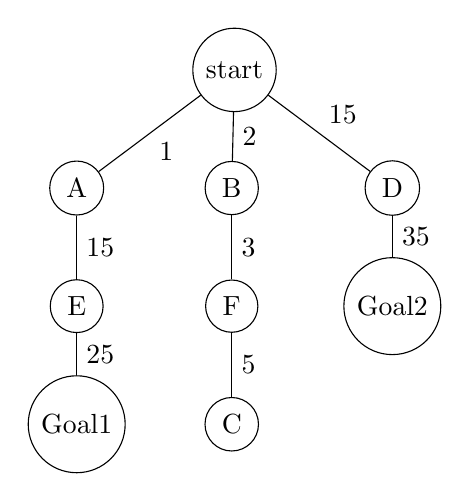
\begin{tikzpicture}[every tree node/.style={draw,circle},
   level distance=1.5cm,sibling distance=1cm,
   edge from parent path={(\tikzparentnode) -- (\tikzchildnode)}]
\Tree
[.start
    \edge node[auto] {1};
    [.A 
       \edge node[auto] {15};
       [.E 
       	\edge node[auto] {25};
       	[.Goal1 ]
       ]
    ]
    \edge node[auto] {2};
    [.B 
        \edge node[auto] {3};
        [.F
		\edge node[auto] {5};
       	[.C ]
         ]
    ]
    \edge node[auto] {15};
    [.D 
        \edge node[auto] {35};
        [.Goal2 ]
    ]
]
\end{tikzpicture}

مسیر رسیدن به هدف
\lr{ start -> D -> Goal2}
می باشد.
\subsection{بخش ب}
اگر هزینه های روی یال ها مهم باشد و هدف کم کردن تعداد گام نباشد خیر زیرا با اجرای الگوریتم هزینه یکنواخت ما به گره \lr{Goal1} می رسیم ولی این بار با هزینه 45 تا می توانیم به گره هدف برسیم در حالی که اکنون با این الگوریتم با هزینه 50 به \lr{Goal2} رسیدیم.

خروجی در صورت اجرای الگوریتم \lr{UCS} به صورت 
\lr{start -> B -> F -> A -> E -> Goal1}
خواهد بود و 
$ g(Goal2) = 45 $

\end{document}




















































